\appendix
\part*{Annexes}
\addcontentsline{toc}{part}{Annexes}
\pagestyle{myheadings}
\markboth{Annexes}{Annexes}

Template LaTeX disponible ici : \url{https://github.com/ChartesHN/}.

Tout mon code est disponible ici : \url{https://github.com/the0phil3/projetMemoire/}.

Le moteur de recherche de la base données du SHD : 
\begin{figure}[h]
    \centering
    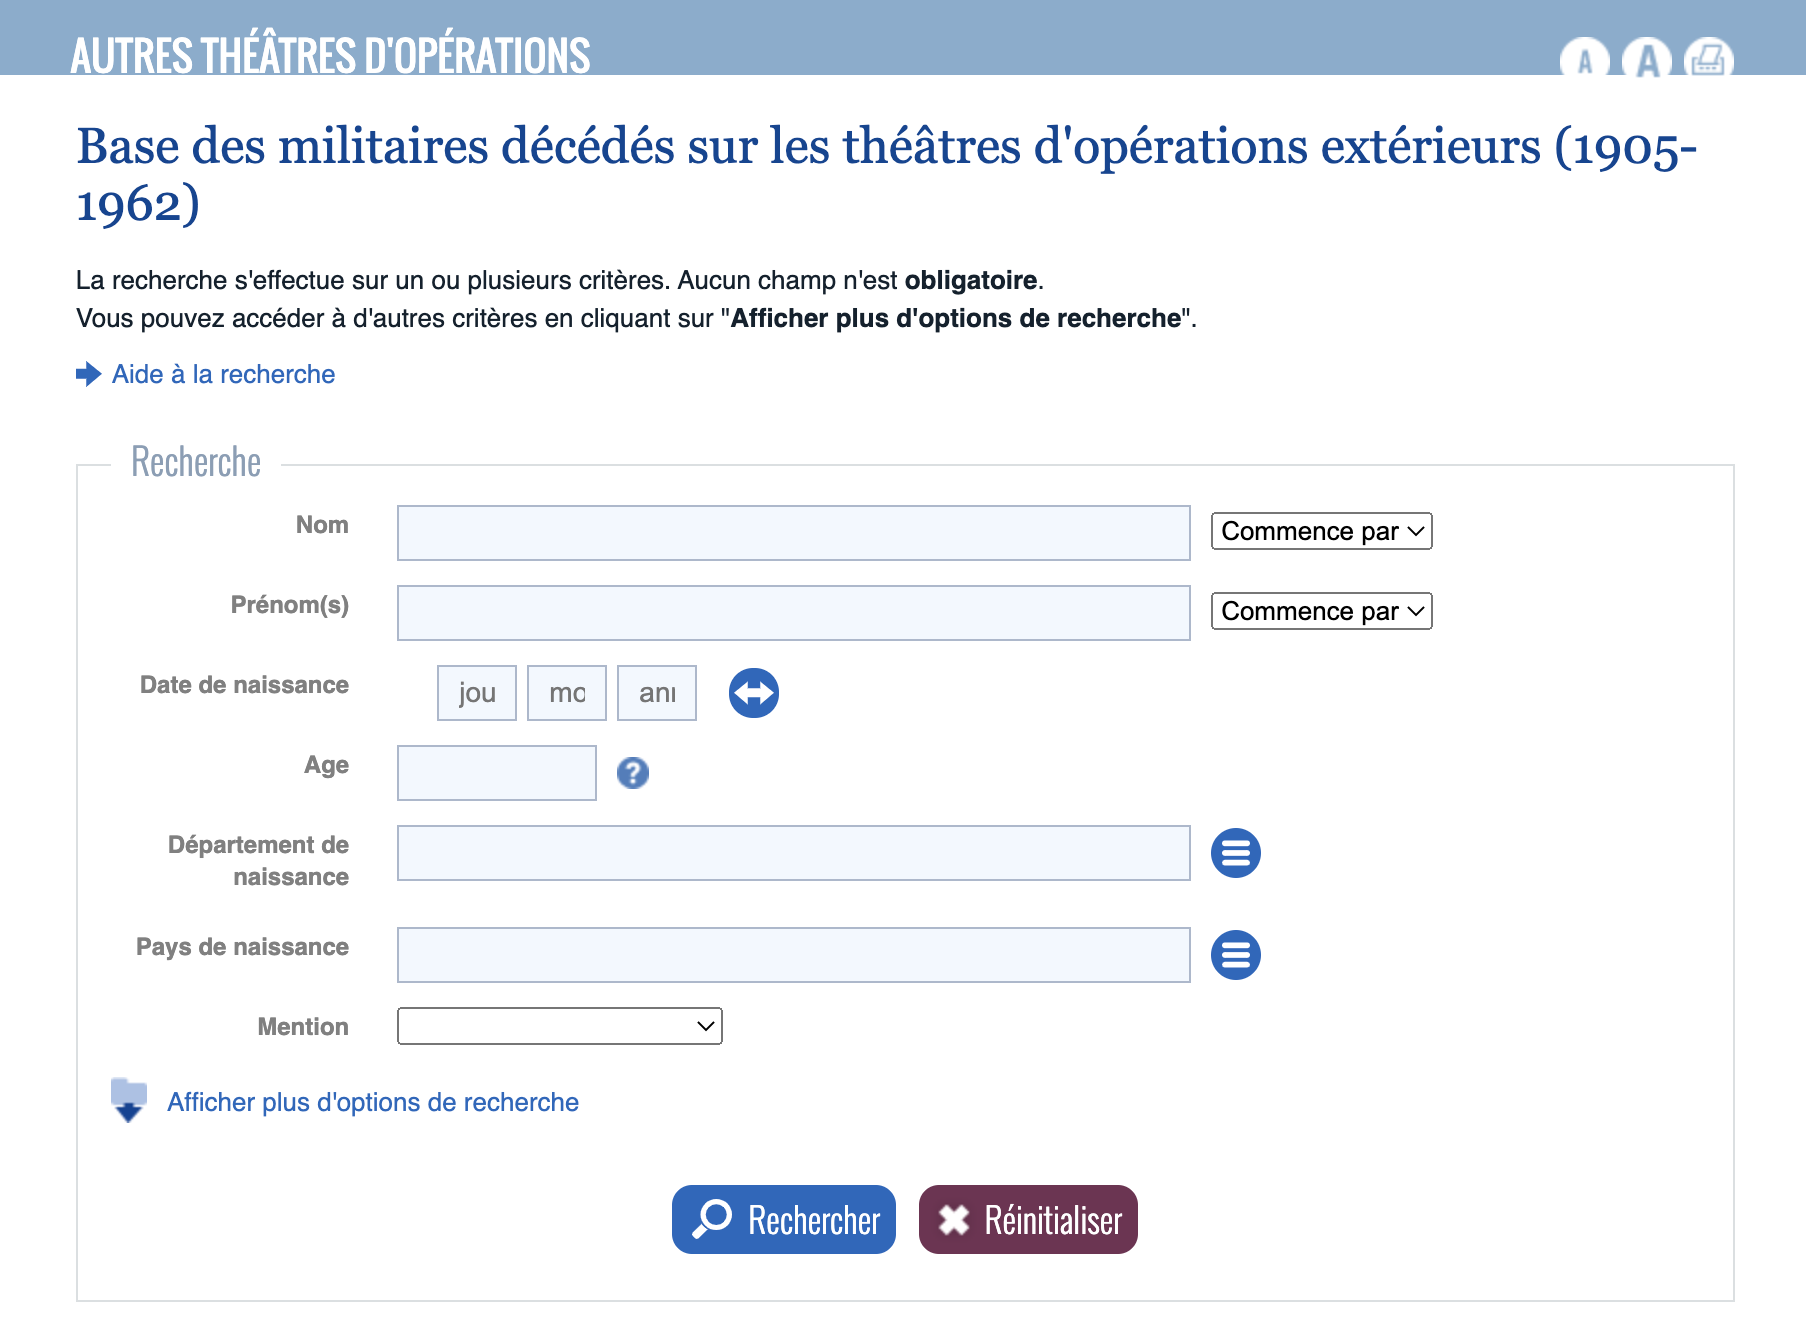
\includegraphics[scale=0.27]{ark1.png}
    \caption{Moteur de recherche simple}
    \label{fig:Arkothèque 1}
\end{figure}
\begin{figure}[h]
    \centering
    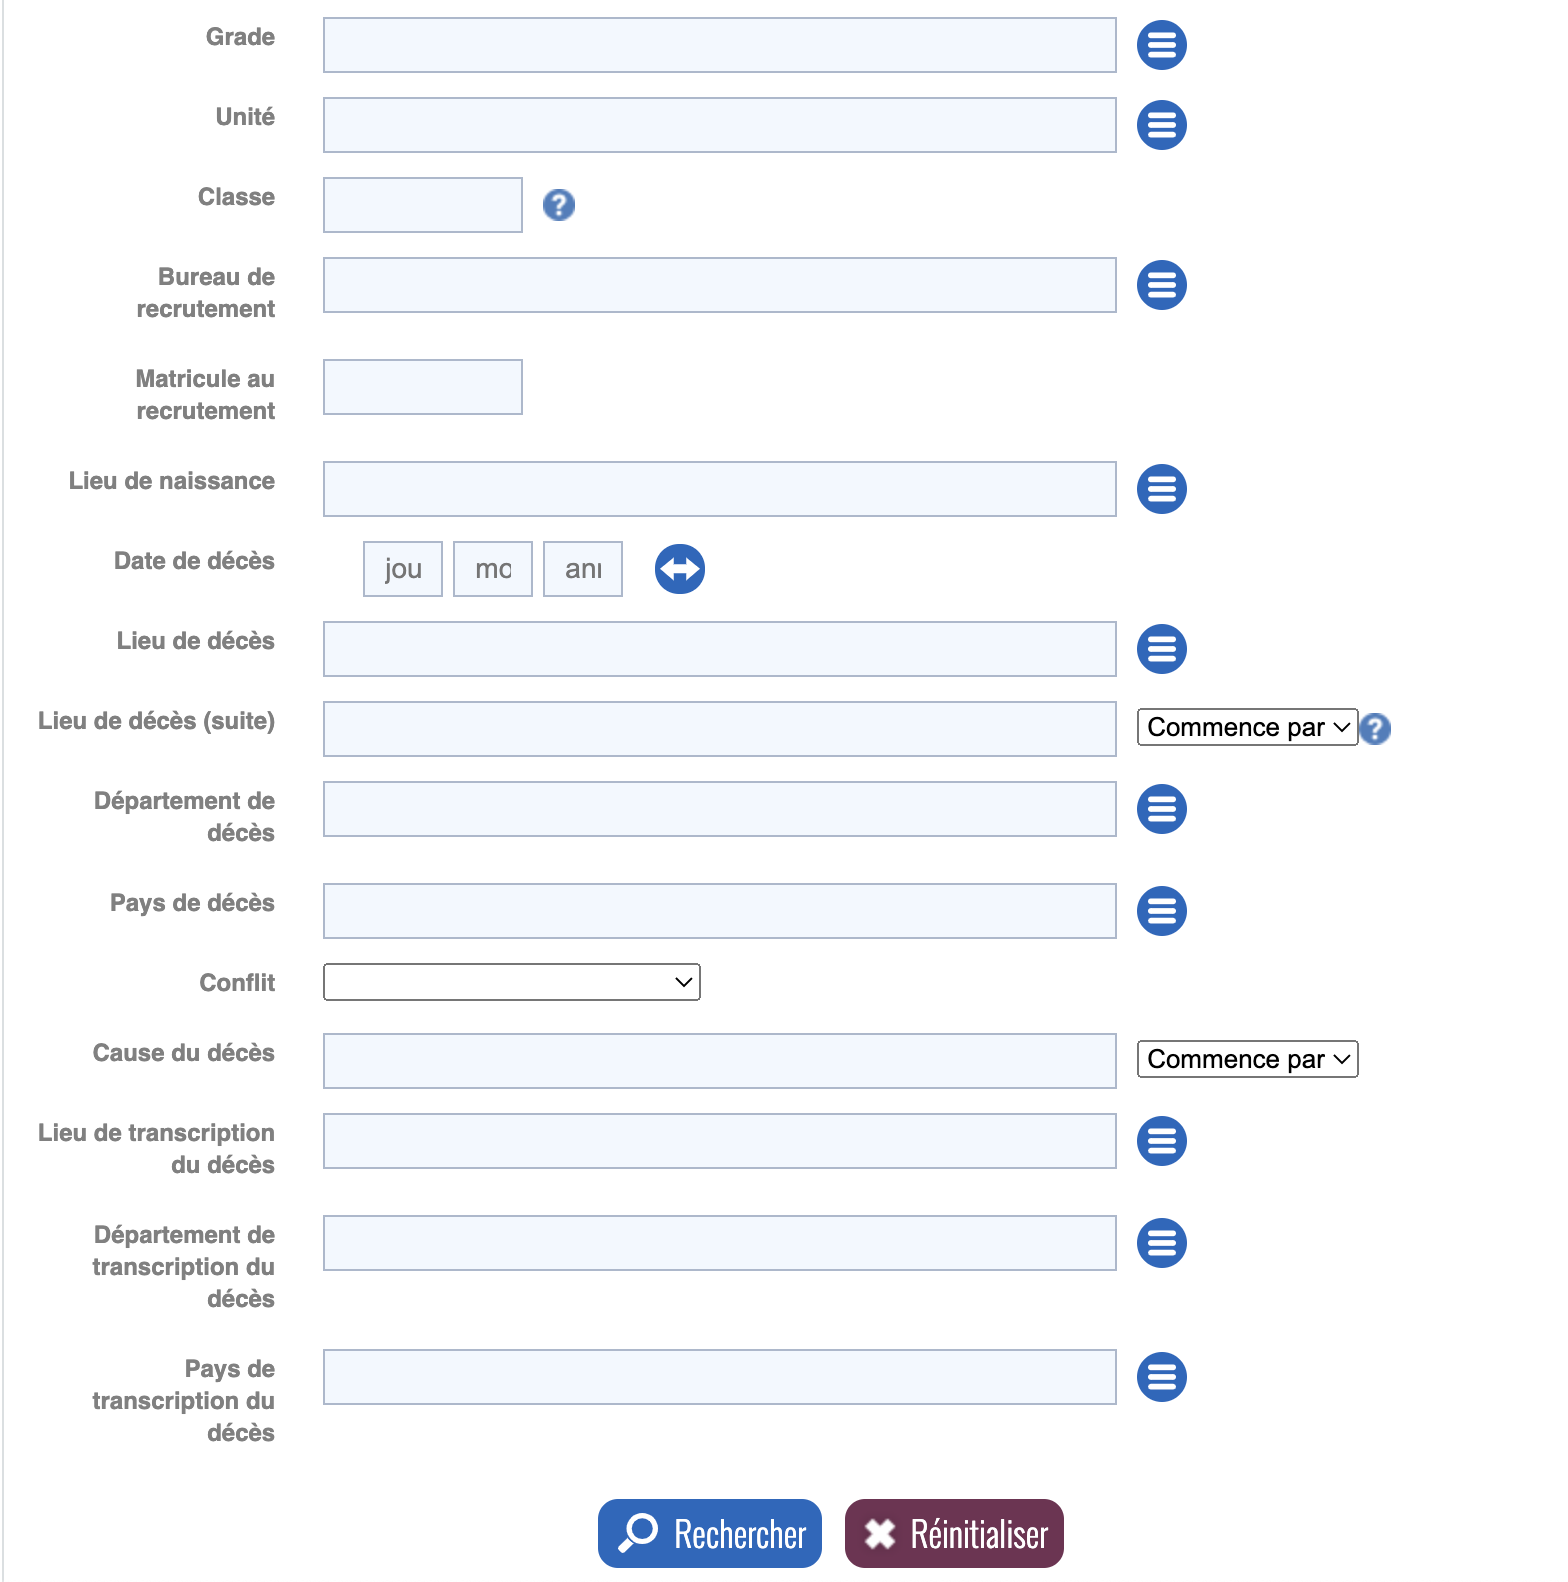
\includegraphics[scale=0.27]{ark2.png}
    \caption{Moteur de recherche avancé}
    \label{fig:Arkothèque 2}
\end{figure}

Le reste de mes resultats: 
\begin{figure}[h]
    \centering
    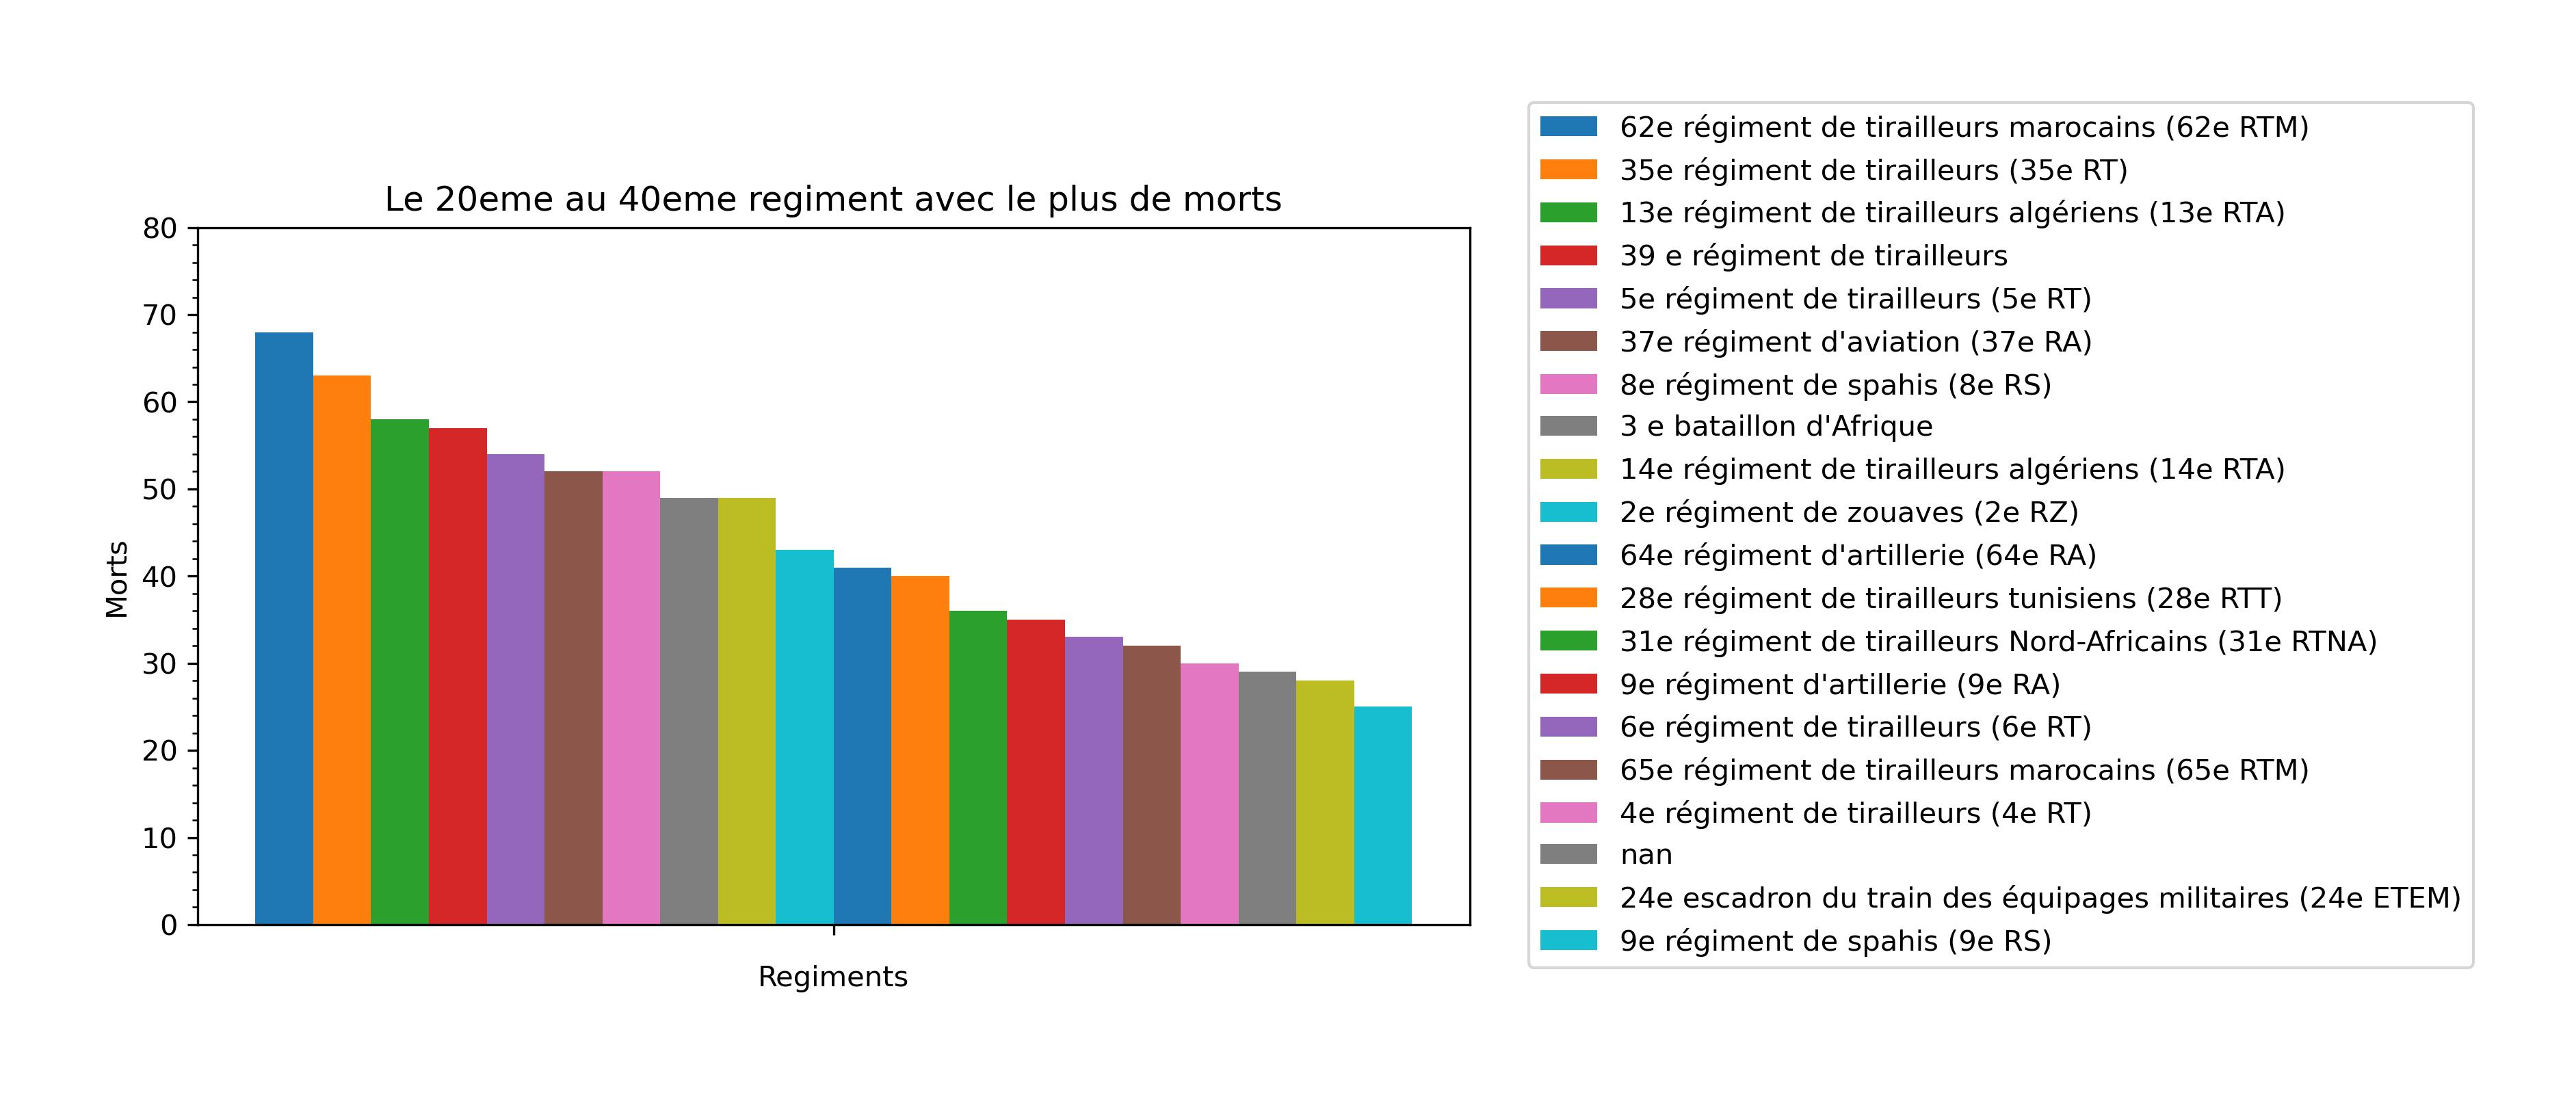
\includegraphics[scale=0.7]{Images/next20regiments.jpg}
    \caption{Les 20 à 40 régiments avec le plus pertes}
    \label{fig:Régiments 2}
\end{figure}
\begin{figure}[h]
    \centering
    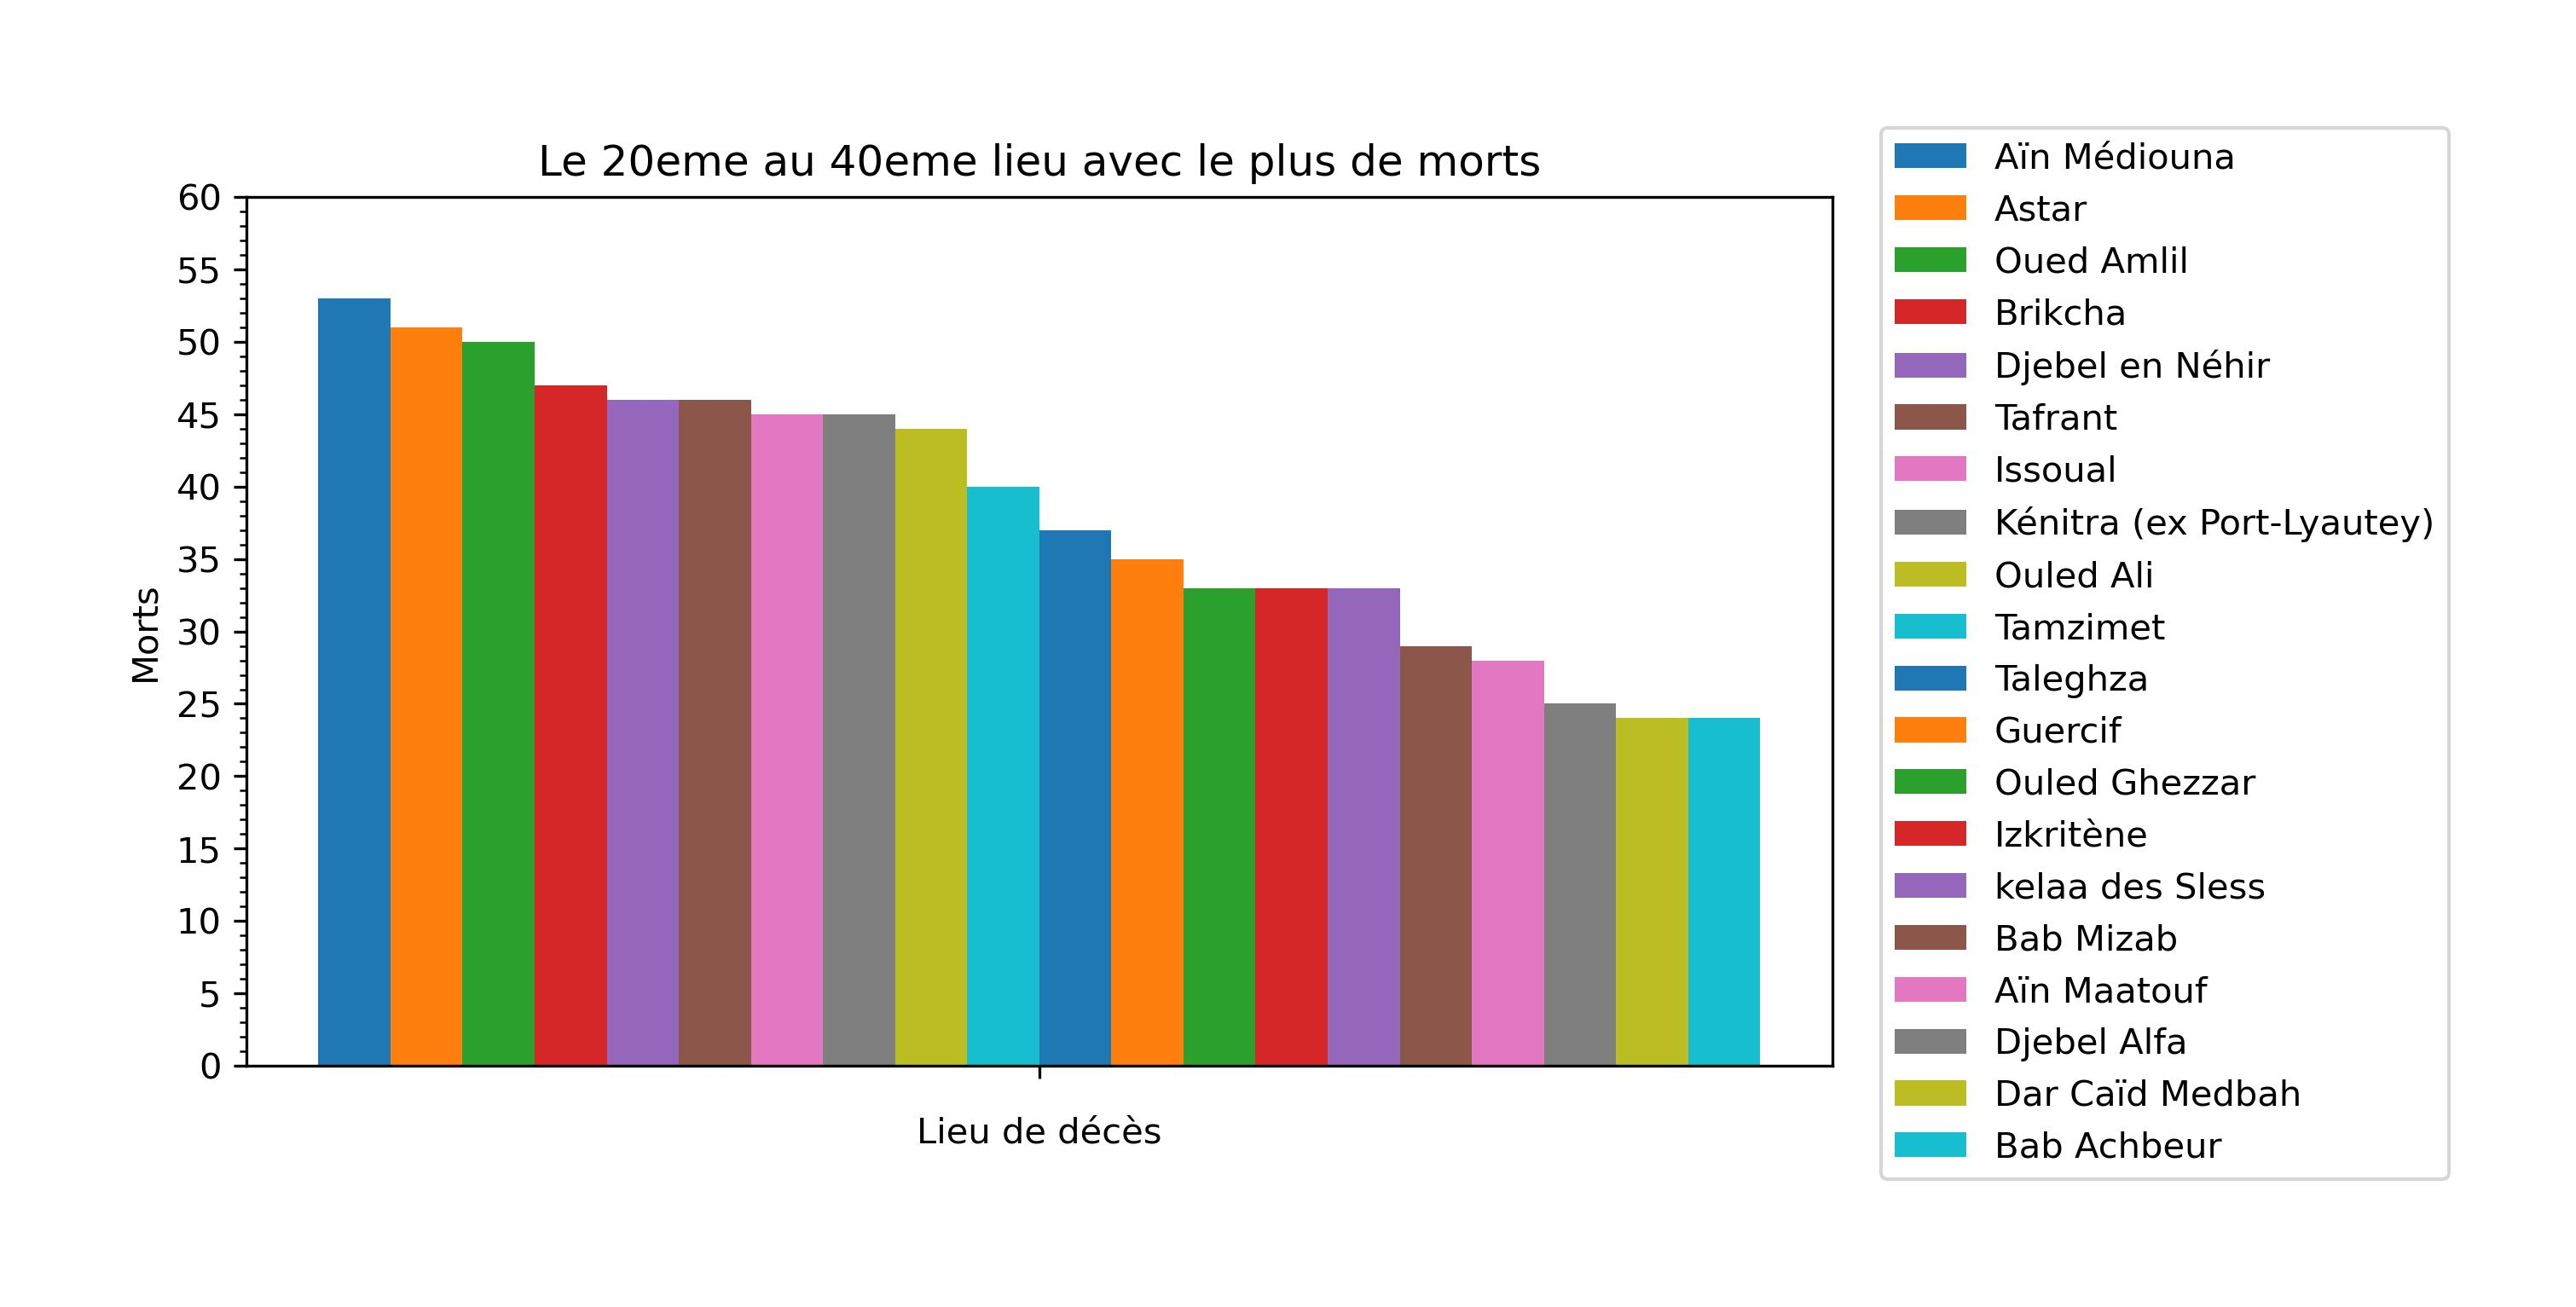
\includegraphics[scale=0.7]{Images/next20places.jpg}
    \caption{Les 20 à 40 lieux avec le plus pertes}
    \label{fig:Lieux 2}
\end{figure}
\begin{figure}[h]
    \centering
    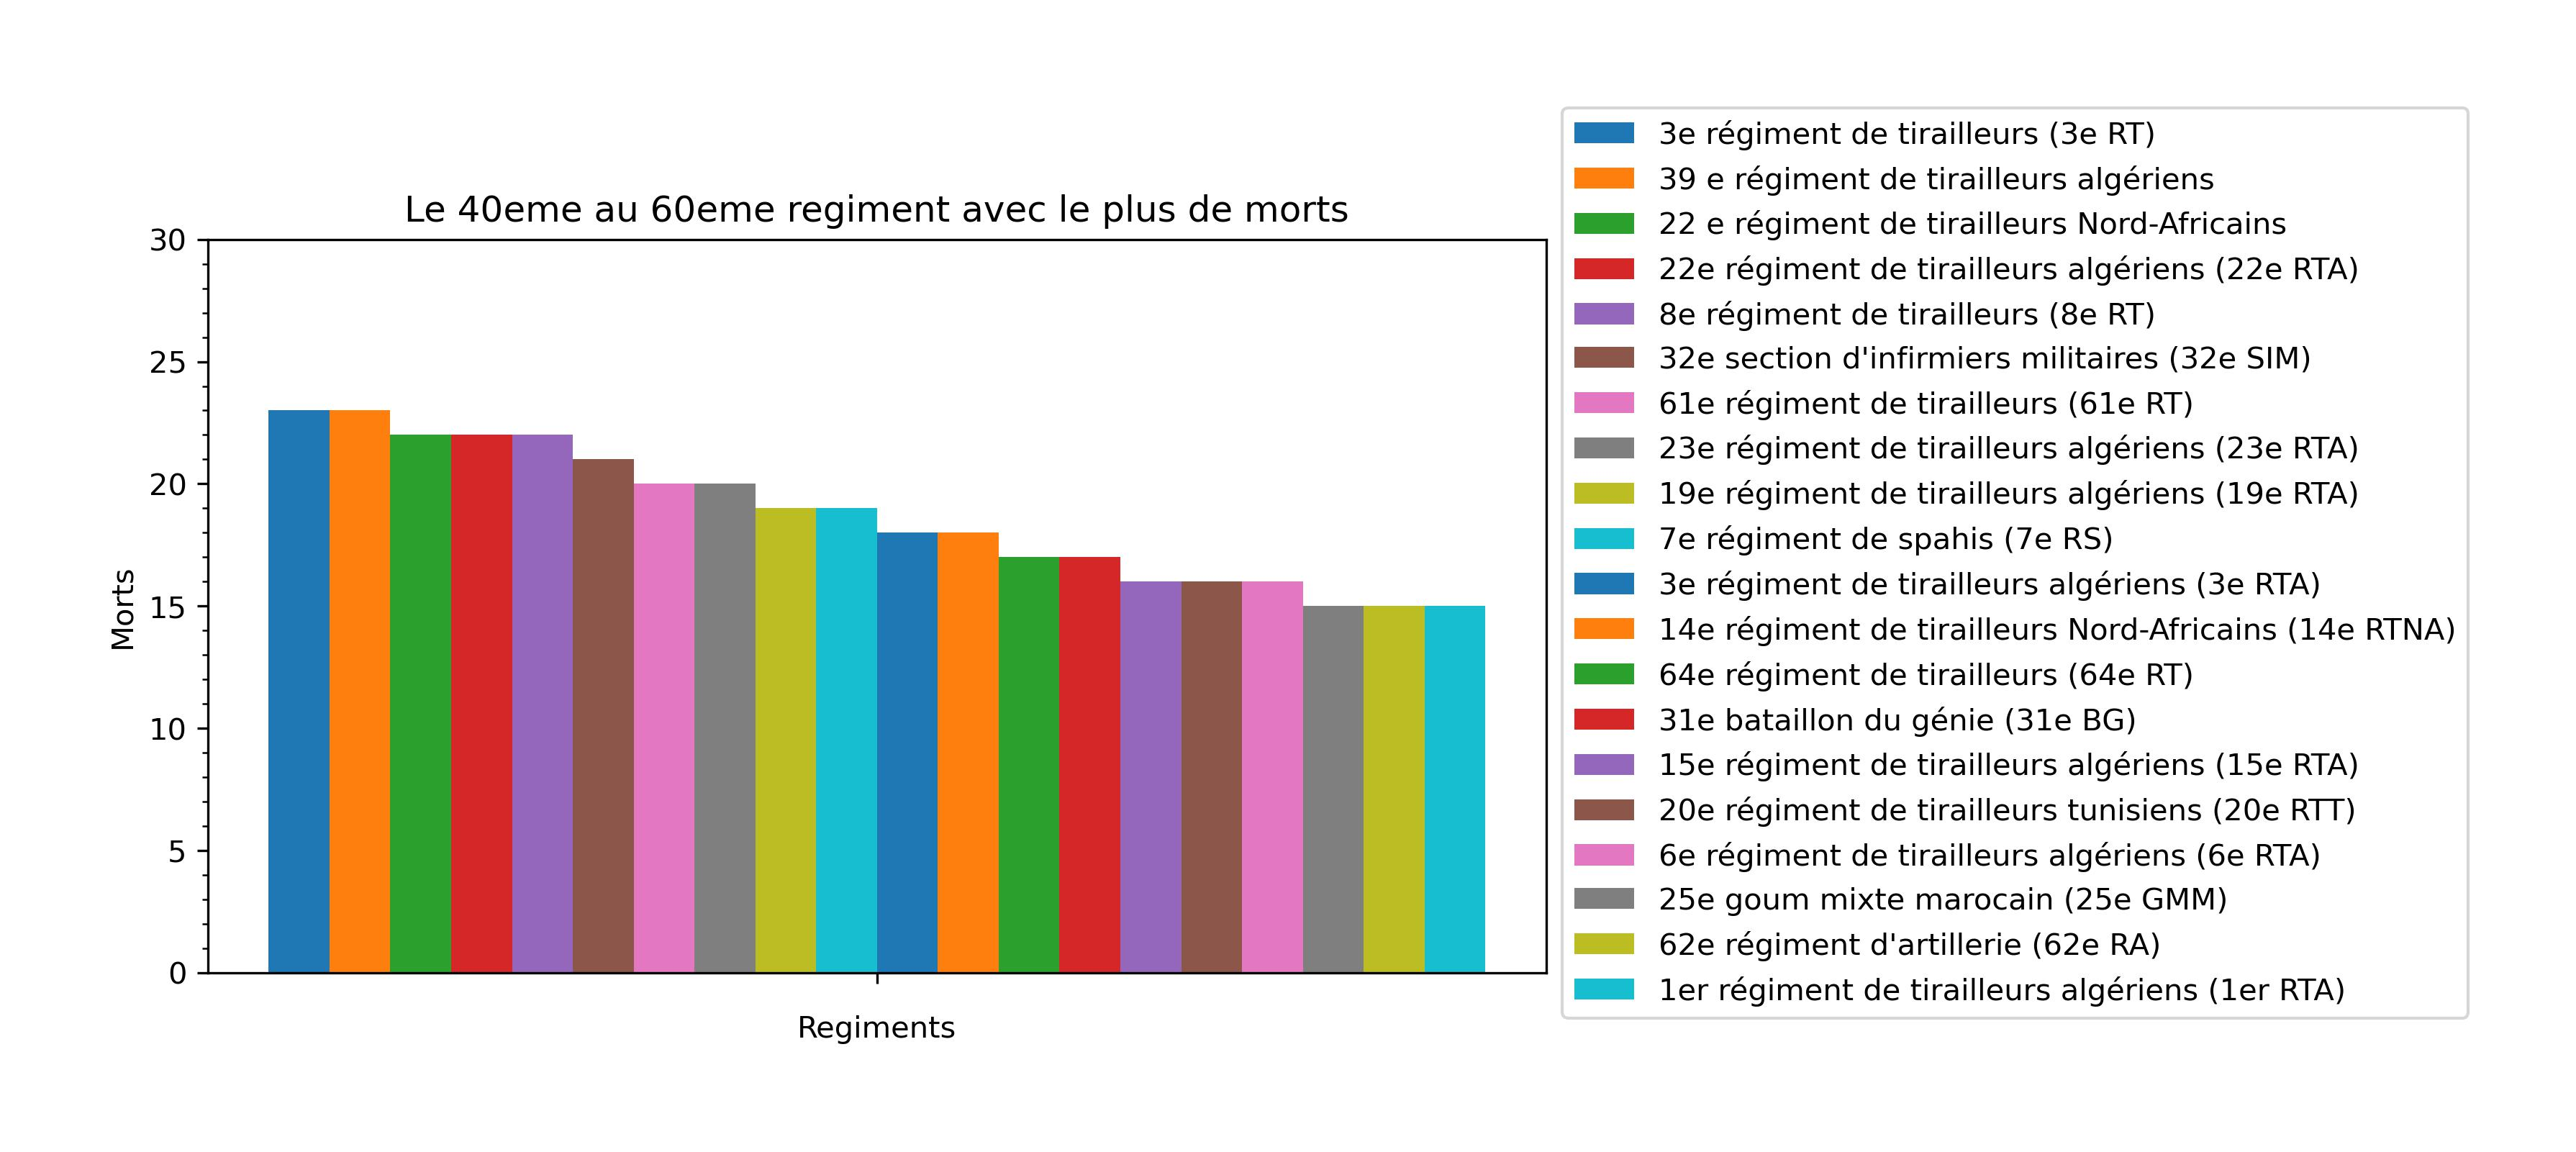
\includegraphics[scale=0.7]{Images/last20regiments.jpg}
    \caption{Les 40 à 60 régiments avec le plus pertes}
    \label{fig:Régiments 3}
\end{figure}
\begin{figure}[h]
    \centering
    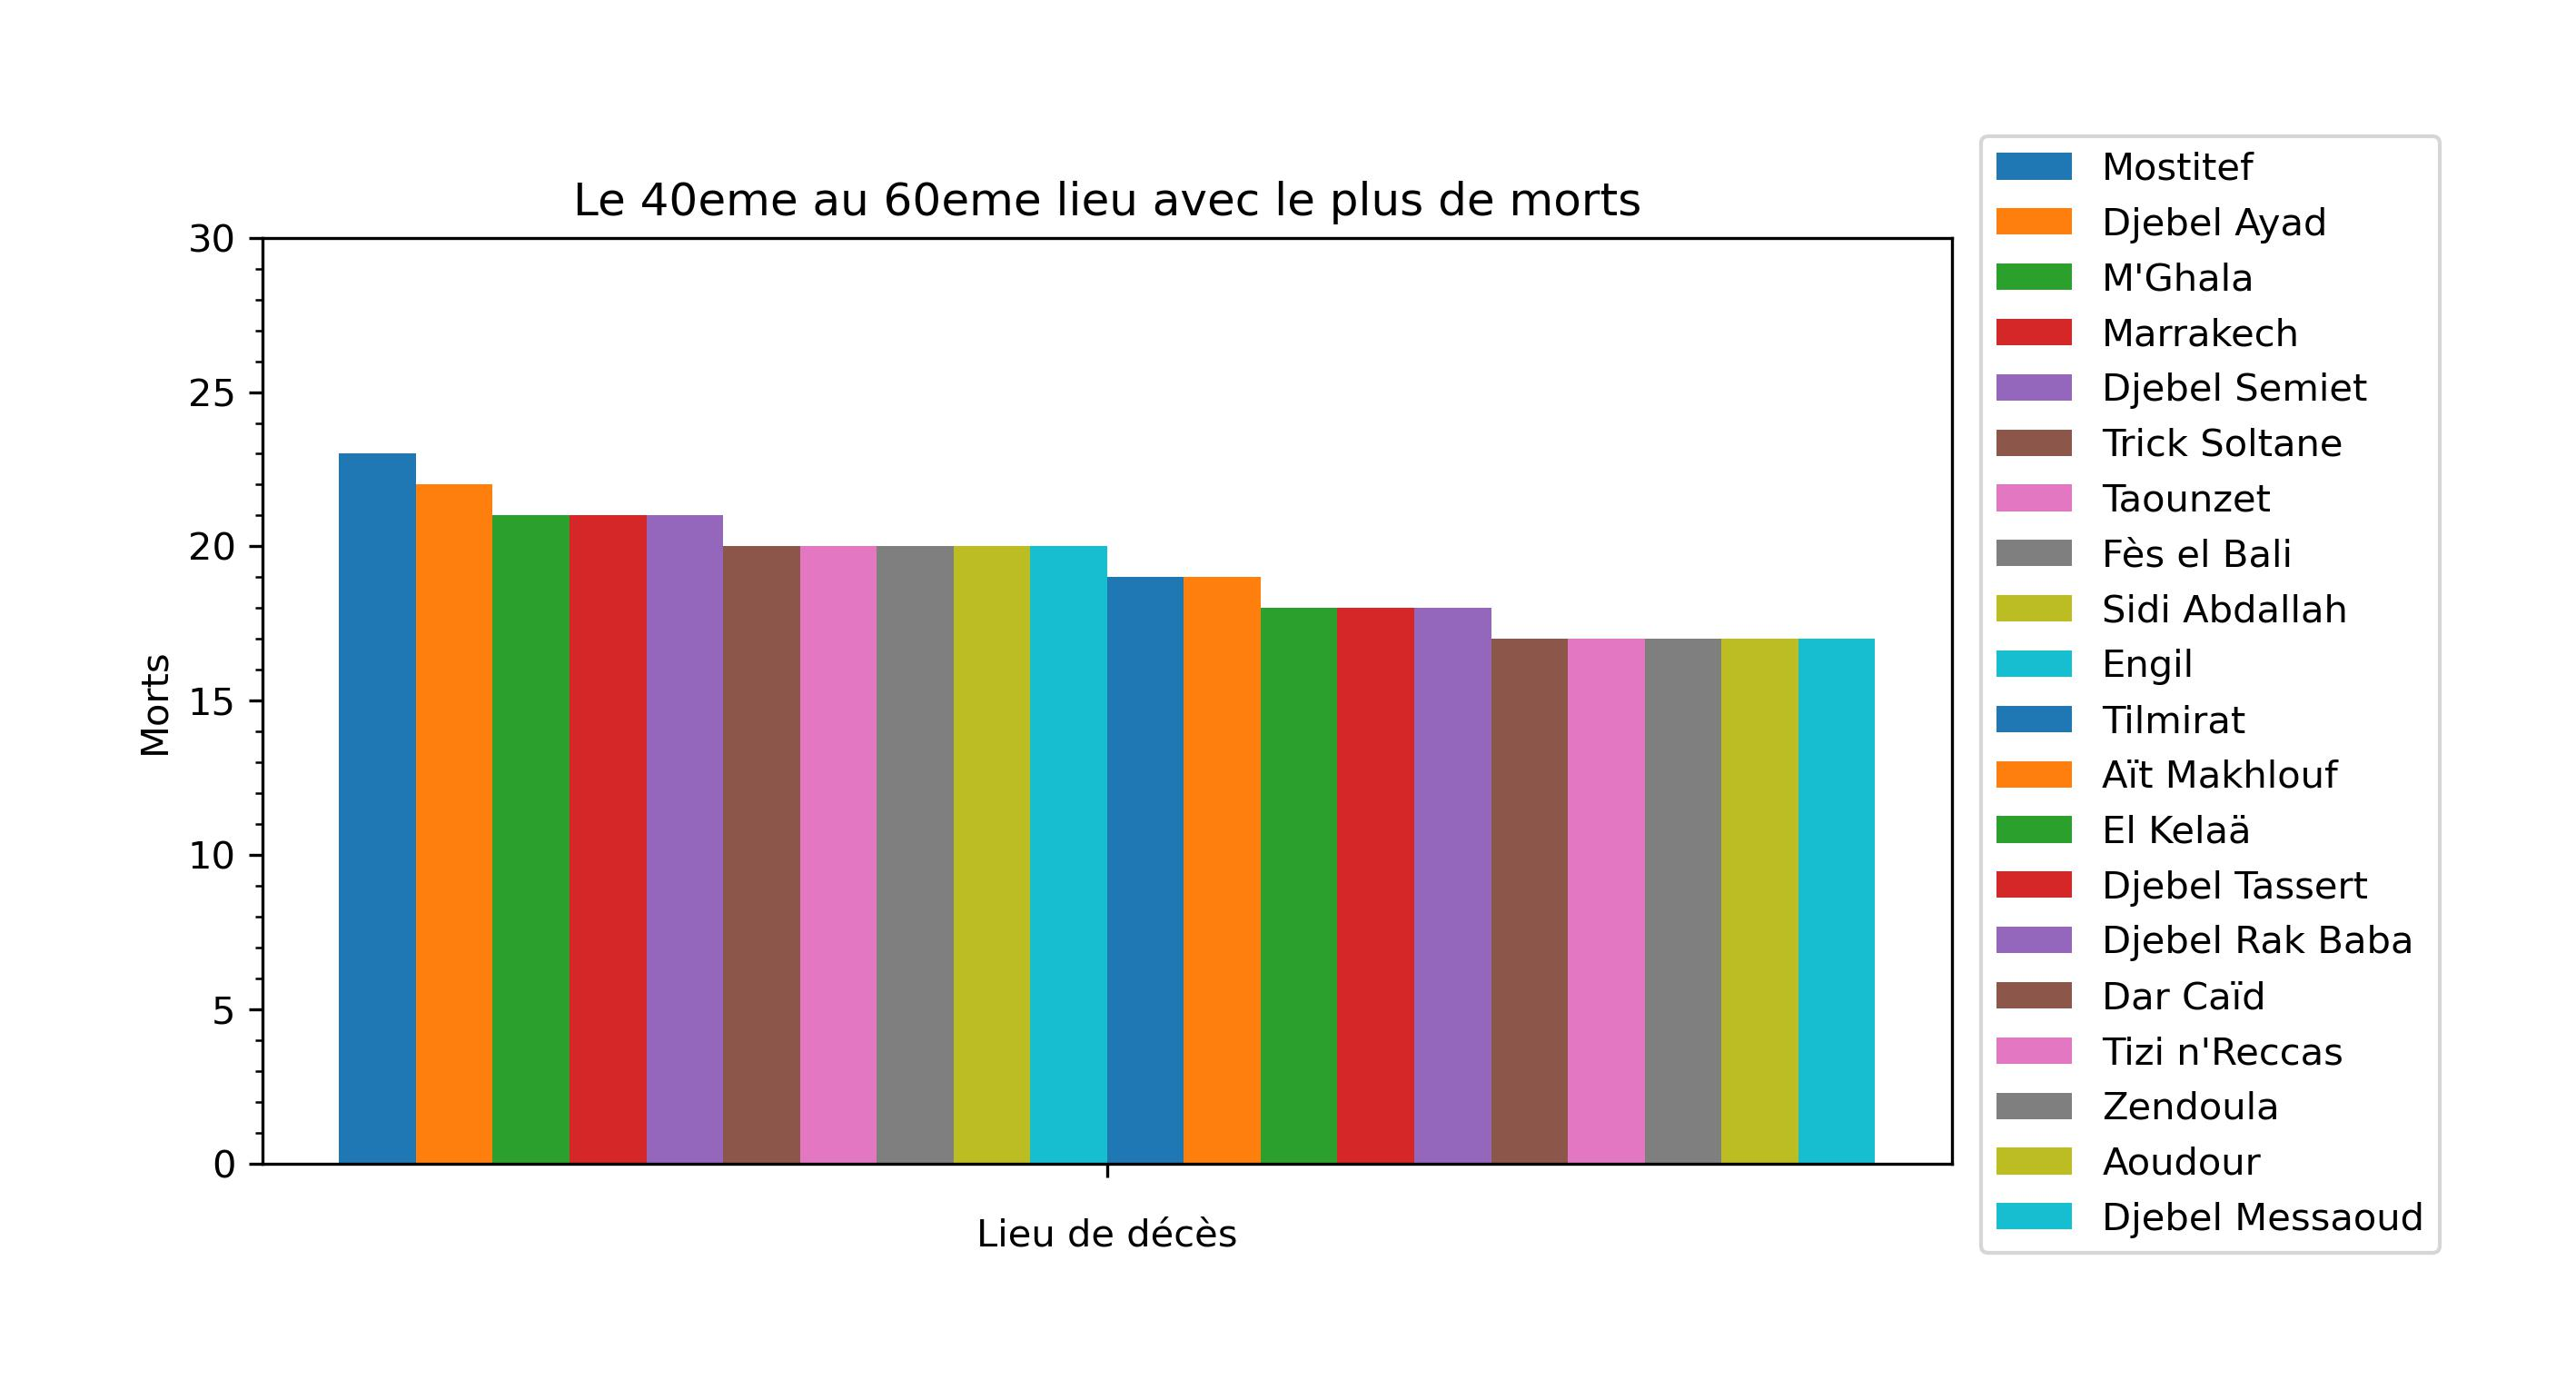
\includegraphics[scale=0.7]{Images/last20places.jpg}
    \caption{Les 40 à 60 lieux avec le plus pertes}
    \label{fig:Lieux 3}
\end{figure}
\begin{figure}[h]
    \centering
    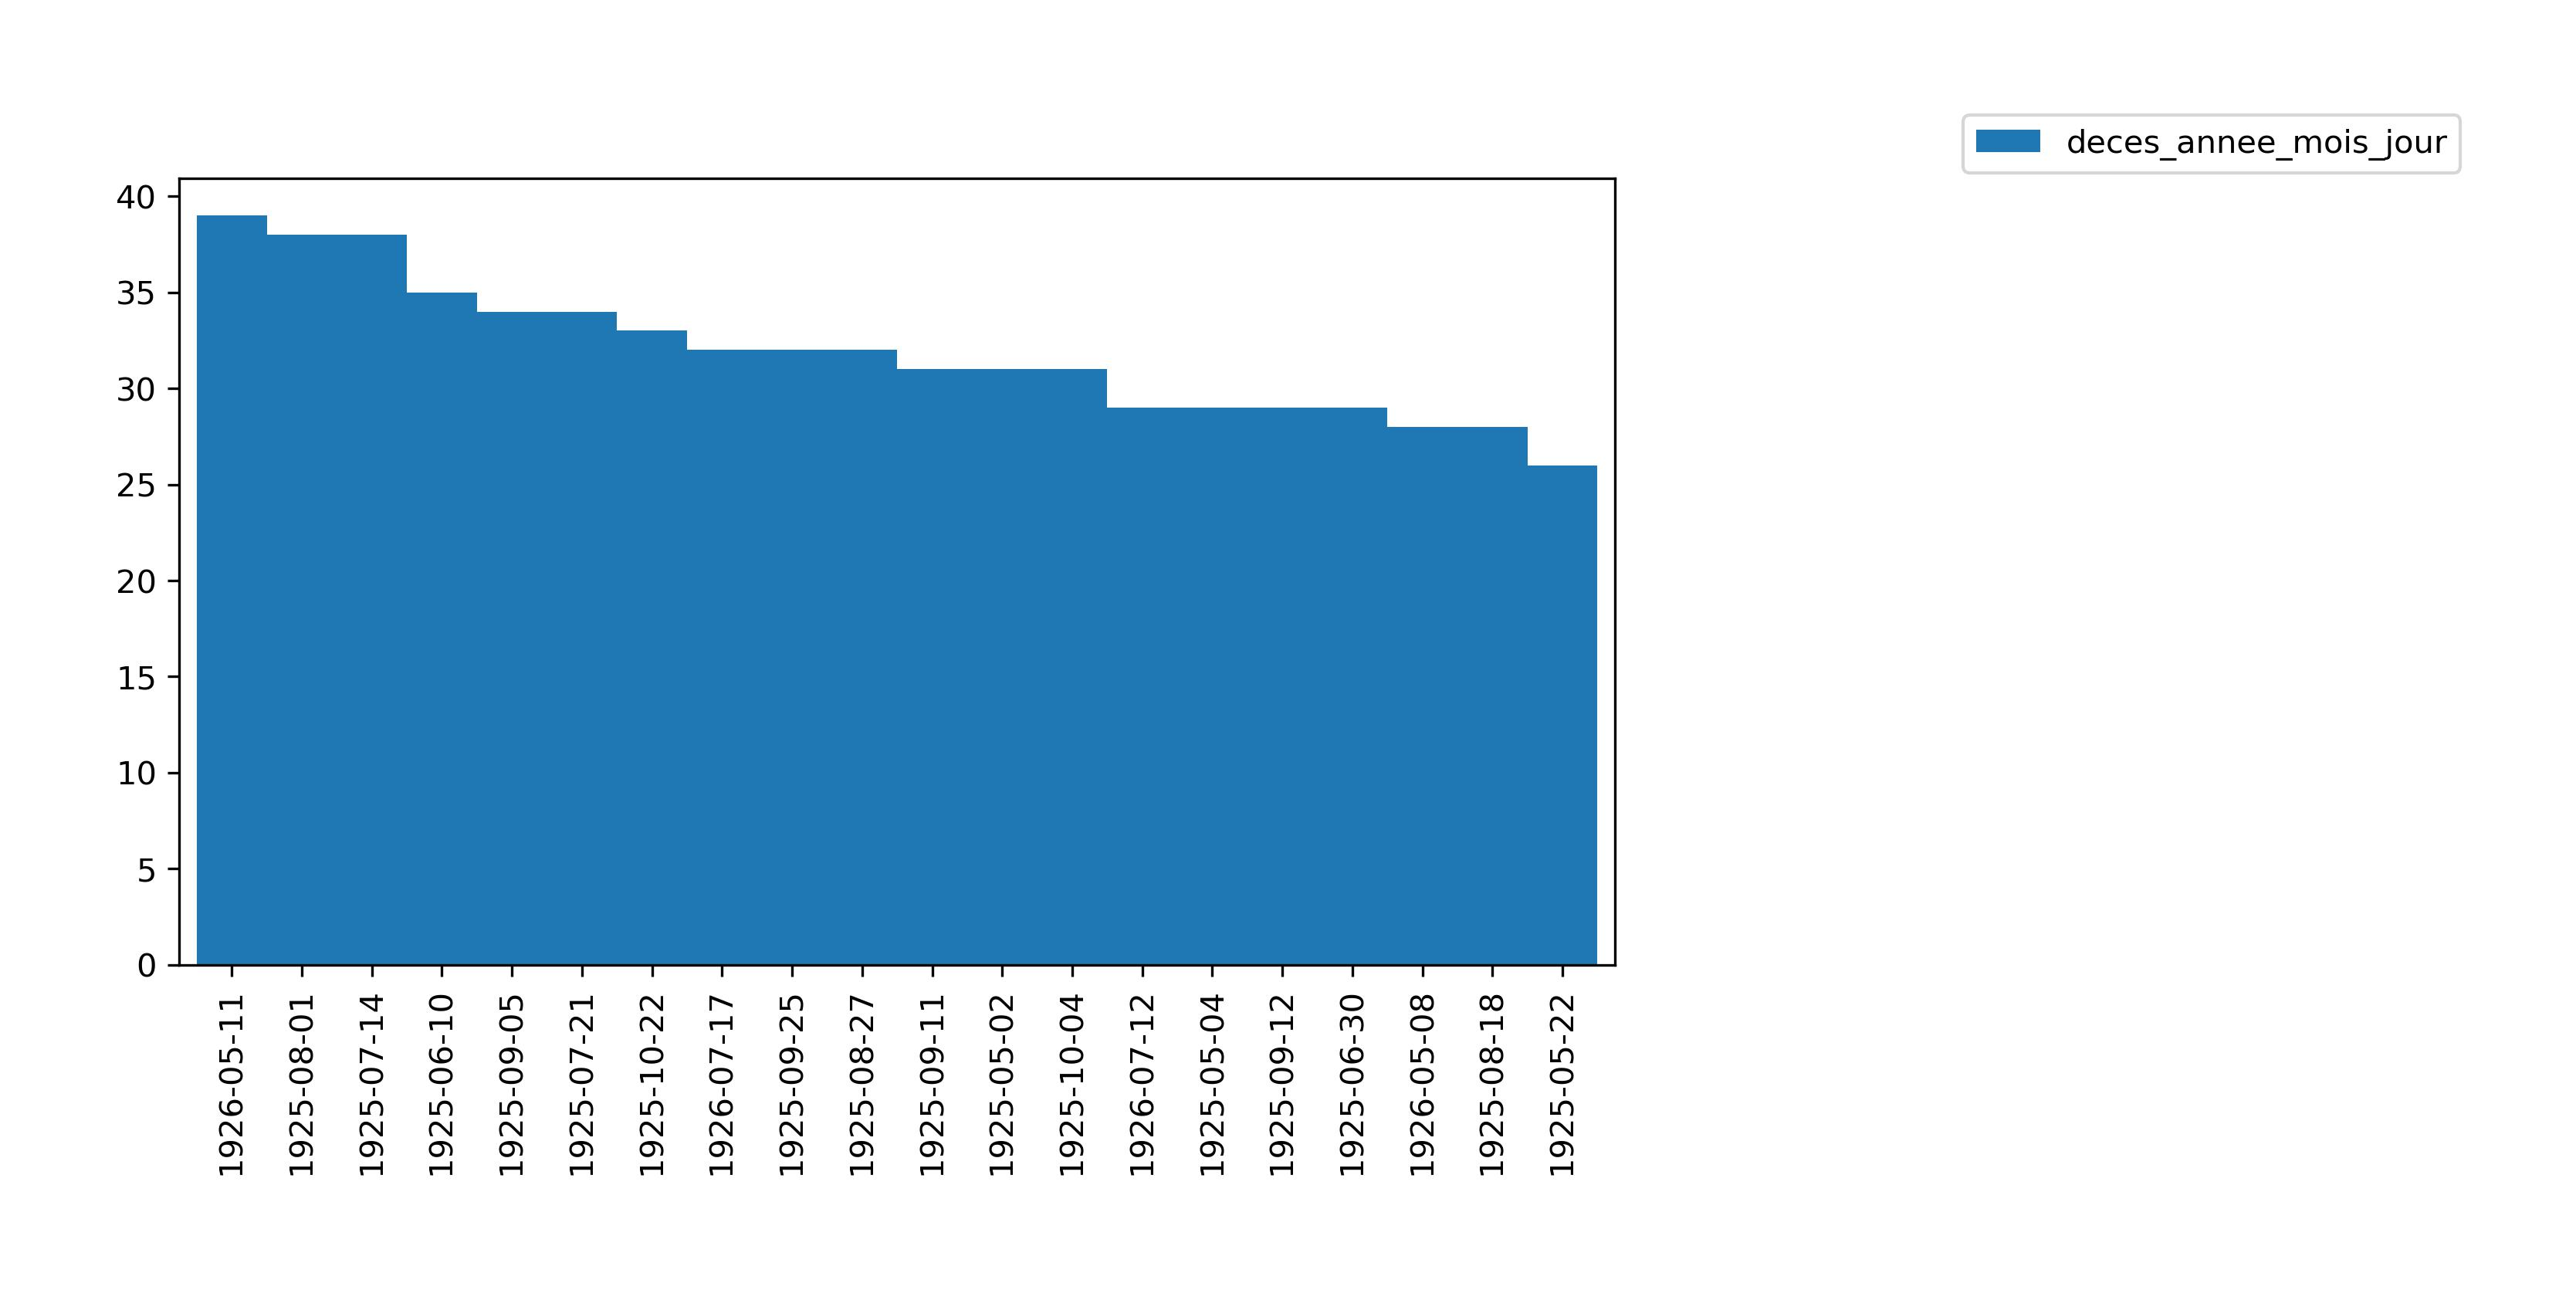
\includegraphics[scale=0.67]{Images/next20dates.jpg}
    \caption{Les 20 à 40 dates avec le plus pertes}
    \label{fig:Dates 2}
\end{figure}